\chapter{Wstęp teoretyczny}

\section{Cel projektu}
Celem projektu było wykorzystanie rozproszonej bazy danych w celu zwiększenia dostępności danych w systemach bibliotecznych.

\section{Zakres projektu}
W zakres projektu wchodziła analiza problemu, dobór technologii oraz rozwiązanie problemu replikacji baz danych. Zbudowanie ekosystemu pozwalającego na replikację oraz obsłużenie go za pomocą load balancera. Aby zbudować ekosystem przeprowadzono gruntowne poszukiwania odpowiedniej technologii pozwalającej na wirtualizację aplikacji oraz ruchu sieciowego oraz planowanie budowy ekosystemu. Na koniec zbudowano oraz skonfigurowano cały ekosystem aplikacji oraz podpięto je do wirtualnej sieci, tak by na zewnątrz pokazać jedynie adres load balancera i poszczególnych aplikacji klienckich (do testów replikacji).

\section{Wymagania funkcjonalne}
W skład wymagań funkcjonalnych systemu wchodzi możliwość przez dwóch aktorów obsługi aplikacji „Księgarni”.\ W zależności od uprawnień aktora można obsłużyć aplikację na dwa sposoby, tak jak pokazuje \refsource{rysunku}{fig:use-case}.

\begin{figure}[H]
    \centering
    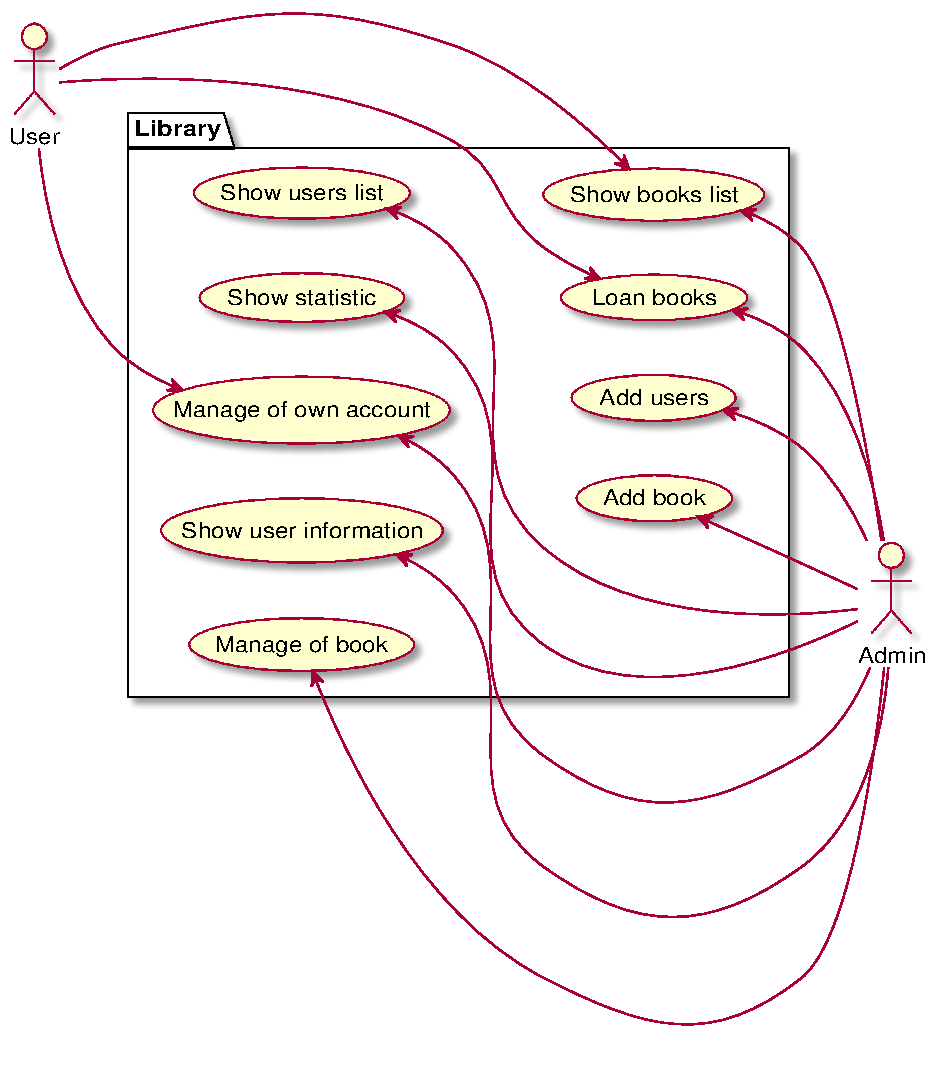
\includegraphics[width=0.5\textwidth]{images/use_case}
    \captionsource{Wymagania funkcjonalne systemu}{Opracowanie własne}
    \label{fig:use-case}
\end{figure}

Użytkownik ma do swojej dyspozycji jedynie przegląd, wypożyczanie książek, a także edycję swoich danych.\ Administrator posiada już więcej możliwości, konto o tej roli pozwala użytkownikowi dodatkowo na zarządzanie książkami oraz oglądanie statystyk wypożyczeń.\ Administrator może również dodawać i usuwać użytkowników oraz przeglądać ich listę.\ Na liście książek, do której również ma dostęp, może przeglądać tytuły ich statystyki oraz modyfikować statusy książek i dodawać ich ''kopie''

\section{Wymagania niefunkcjonalne}
W skład wymagań niefunkcjonalnych wchodzi technologia jaka została wykorzystana do stworzenia środowiska potrzebnego do sprawdzenia możliwości replikacji bazy PostgreSQL \cite{Pos2023}.\ Do jej obsługi skorzystano aplikacji klienckiej napisanej w języku PHP 7.4 \cite{Php2023}, przy użyciu frameworka Symfony 5 \cite{Sym2023}.\ Całość została uruchomiona za pomocą kontenerów Dockerowych \cite{Doc2023}, całość została obsłużona przez konfigurację napisaną przy użyciu biblioteki dla Docker: Docker Compose.\ Dodatkowo Load Balancer został uruchomiony na serwerze Nginx \cite{Nginx2023}.\ Wszystkie kontenery zostały wpięte do wirtualnej sieci utworzonej przez Dockera.\ Schemat aplikacji został zaprezentowany na \refsource{obrazie}{fig:roisb}.

\begin{figure}[H]
    \centering
    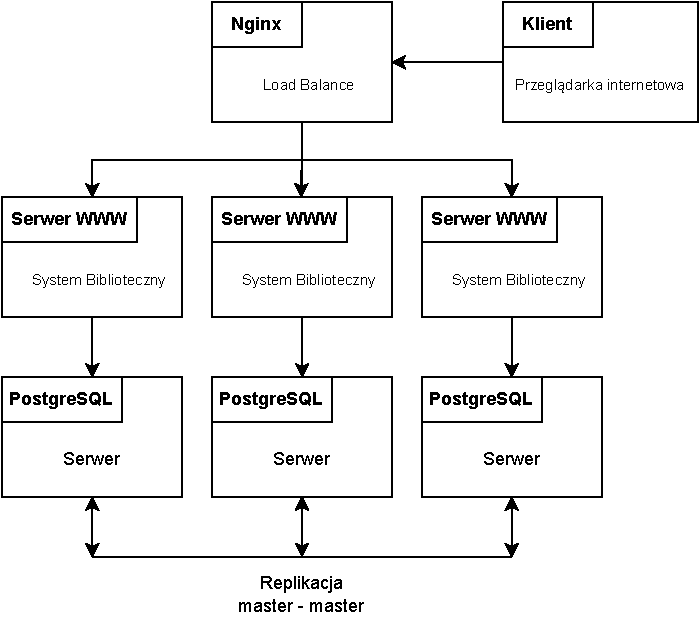
\includegraphics[width=0.5\textwidth]{images/roisb}
    \captionsource{Schemat ekosysteu apikacji}{Opracowanie własne}
    \label{fig:roisb}
\end{figure}
